\documentclass[pdflatex,sn-mathphys-num]{sn-jnl}
\usepackage{graphicx}
\usepackage{multirow}
\usepackage{amsmath,amssymb,amsfonts}
\usepackage{booktabs}
\usepackage{textcomp}
\usepackage{xcolor}
\usepackage{url}
\graphicspath{{figures/}{./}}
\newcommand{\sysname}{SignalCheck}
\raggedbottom

\begin{document}
\title[\sysname{} Revisited]{\sysname{} Revisited: Benchmark Artefacts and Modality Scope in Bangla Fake-News Image Detection}

\author*[1]{\fnm{Given} \sur{Name}}\email{author@example.com}
\affil*[1]{\orgdiv{Department}, \orgname{Institution}, \orgaddress{\city{City}, \country{Bangladesh}}}

\abstract{Fake news detection for low-resource languages such as Bangla depends on
synthetically constructed benchmarks, and a constructed benchmark is assembled
by a pipeline that leaves traces. This paper reports an image-level detector
for manipulated Bangladeshi news imagery together with the controls needed to
say what its numbers mean. Two properties of the BanFakeMM benchmark change the
interpretation of any result obtained on it. First, file metadata
alone---resolution, format and colour mode, with no pixel content---separates
manipulated from authentic images at 100 percent accuracy; re-encoding every
image through one identical pipeline removes the artefact at a cost of
1.03 accuracy points, which establishes that the remaining signal lies in the
content; a weaker version of the same shortcut (77 to 83 percent) appears in a
second Bangla corpus. Second, the benchmark's five attack types do not pose a single task:
in three of them every one of the 1,000 manipulated images is byte-identical to
an authentic image, so an image-only model is undecidable there, and its
measured AUROC on those splits is 0.48 to 0.52. We scope the evaluation to the
two splits in which the manipulation reaches the pixels. Within that scope, a
per-modality ablation under duplicate-aware grouped cross-validation shows CLIP
visual features dominating at 95.38 percent---94.35 with the artefact
removed---while every text-only configuration saturates below 78 percent; OCR
and the caption-fusion pathway are removed on evidence rather than by
assumption. Transfer to an unseen manipulation style costs roughly nine points
of accuracy on a 1,308-image sealed partition, and supervised adaptation on
300 target-style images improves ranking by 0.025 AUROC, with confidence
intervals excluding zero across eight seeds and both encodings. Two conclusions
we previously published about this system---that the shift penalty was largely
a calibration effect, and that supervised adaptation added nothing---are
corrected here, together with the measurements that force the correction.}

\keywords{Bangla fake news detection, multimodal misinformation, CLIP, distribution shift, dataset artefacts, shortcut learning, near-duplicate leakage, evaluation methodology, low-resource language processing}

\maketitle



%==============================================================
% INTRODUCTION + RELATED WORK -- journal version.
%
% Rewritten against the conference version because the contributions changed:
% the benchmark decomposition and the artefact control are new, and two of the
% conference version's own conclusions are corrected here.
%
% THREE NEW REFERENCES, each verified against a machine-readable record:
%   shortcut     Geirhos et al., Nature Machine Intelligence 2020,
%                doi:10.1038/s42256-020-00257-z  (arXiv:2004.07780)
%   datasetbias  Torralba & Efros, CVPR 2011, pp. 1521-1528,
%                doi:10.1109/CVPR.2011.5995347
%   nadeau       Nadeau & Bengio, Machine Learning 52(3), 2003, pp. 239-281,
%                doi:10.1023/A:1024068626366
% Bibitems for all three are at the end of this file.
%==============================================================

\section{Introduction}

Bangladesh's social media ecosystem has become a primary vector for manipulated
news imagery, from digitally altered photocards and forged documents to
AI-generated video frames misattributed to public figures. Unlike text-only
misinformation, this content exploits the visual and textual channels jointly:
a viral image is judged not on its pixels alone but on the claim attached to it
as it spreads.

The problem is compounded by linguistic specificity. Most fake-news detection
methods are built on English datasets from Western platforms and presuppose
signals---dense comment threads, public retweet graphs---that are sparse or
structured differently in Bangladesh. No large-scale, organically collected
corpus of manipulated Bangladeshi news images exists, so training must rely on
synthetically constructed benchmarks.

That reliance is the starting point of this paper. A constructed benchmark is
reproducible, which is its virtue, but it is also assembled by a pipeline, and
a pipeline leaves traces. Two consequences follow, and neither is checked as a
matter of course. First, the classes may be separable for reasons that have
nothing to do with the phenomenon under study: if the generator emits images at
one resolution and the authentic images arrive at many, a model can score
perfectly without looking at a picture---the shortcut-learning failure
\cite{shortcut} in the form dataset-bias work has warned about for over a
decade \cite{datasetbias}, and which audits of fake-news corpora have since
found in practice \cite{verma}. Second, a benchmark that advertises several
``attack types'' may not pose the same task in each of them: if an attack
rewrites an article's text and reuses its photograph unchanged, then an
image-only model is being asked a question whose answer is not present in its
input, and whatever number it produces is not a measure of its competence. A
related concern, unimodal bias, has been documented in English multimodal
misinformation benchmarks \cite{verite}.

We find both in BanFakeMM \cite{banfakemm}, the benchmark this work builds on,
and both change what the surrounding results mean. This paper therefore reports
a detector and, inseparably, the measurement discipline needed to say anything
about it.

Our contributions are as follows.

\begin{itemize}
\item \textbf{A decomposition of the benchmark by modality.} Of BanFakeMM's
five adversarial splits, two manipulate the image and three manipulate the
article text while reusing the photograph: in each of those three, every one
of the 1{,}000 manipulated images is byte-identical to an authentic image from
the benchmark's own corpus. An image-only detector is well posed on two splits
and undecidable on three, and we show its measured behaviour matches that
prediction to the decimal.

\item \textbf{A dataset artefact, and a control that it survives.} In the
training split every manipulated image shares one resolution, and a classifier
given only file metadata---no pixels---separates the classes perfectly.
Re-encoding every image through one identical pipeline removes the artefact and
costs the visual model $1.03$ accuracy points, which establishes that the
signal is in the content.

\item \textbf{A per-modality ablation under duplicate-aware grouped
cross-validation}, which removes OCR on evidence rather than by assumption and
shows the caption-fusion pathway does not earn its computational cost, together
with a like-for-like comparison against the feature families of the closest
prior Bangla multimodal system under that same protocol.

\item \textbf{A distribution-shift evaluation} on a 1{,}308-image sealed
partition---$6.7\times$ the one used in earlier work on this system---with the
artefact controlled, thresholds selected on a disjoint partition, and
article-level overlap measured rather than assumed away.

\item \textbf{Evidence that supervised adaptation helps}, and an account of why
an earlier measurement said otherwise. Adaptation on 300 target-style images
improves ranking by $+0.025$ AUROC with confidence intervals excluding zero
across eight seeds, in both the controlled and uncontrolled settings. The
earlier null rested on accuracy at a fixed threshold on 194 images from a
single fit---a statistic we show can disagree in sign with the effect it is
meant to measure.
\end{itemize}

Two of these findings correct conclusions we previously published about this
same system. We state them as corrections, with the measurements that force
them, rather than quietly revising the numbers.

We claim no architectural novelty. BLIP/CLIP feature extraction with a
gradient-boosted classifier is well established, and the accuracy it reaches
here is unremarkable. What we have not found in the Bangla literature is an
image-level manipulation detector whose reported numbers are accompanied by
evidence that the benchmark supports them.

\section{Related Work}

\subsection{Bangla Fake News Detection}

Research on Bangla-language fake news detection remains limited relative to
English. BanFakeNews \cite{banfakenews} established an early large-scale
benchmark of roughly 50{,}000 Bangla news items labeled authentic or
fabricated, and BanFakeNews-2.0 \cite{banfakenews2} extended that line to a
60{,}000-instance curated corpus with an LLM-based benchmark. Both are
text-only. MultiBanFakeDetect \cite{multibanfake} moved to multimodal
settings with a hybrid DenseNet-169/mBERT fusion architecture and is the
closest prior system to the present work in both language and modality scope.
Beyond Bangla specifically, MMCFND and its MMIFND dataset \cite{mmcfnd} extend
caption-aware detection to seven low-resource Indic languages including
Bengali.

None of these is organised around a defined image-manipulation task with
adversarially constructed positive examples: MultiBanFakeDetect labels whole
articles by their overall claim, so a model may succeed on textual cues alone,
and the remaining systems do not take images as a decision input at all. This
is the gap BanFakeMM \cite{banfakemm} addresses and the one we work in---with
the qualification, established in Section~\ref{sec:detectable}, that only part
of that benchmark poses an image-level task.

\subsection{Multimodal Misinformation Detection}

Outside the Bangla literature, EANN \cite{eann}, MVAE \cite{mvae} and SpotFake
\cite{spotfake} established that visual and textual signals are complementary
for misinformation detection, each on English-language, Western-platform data.
A more recent line pairs multimodal classification with retrieval-augmented,
multi-model verification---DEFAME \cite{defame}, RAGAR \cite{ragar}, RAMA
\cite{rama} and CaLM \cite{calm}---and reports gains from grounding a verdict
in retrieved evidence rather than in the classifier alone. None is
Bangla-specific or grounded in a Bangladeshi corpus. We do not evaluate a
verification stage here; Section~\ref{sec:limitations} explains what
evaluating one properly would require and why we judge our preliminary
measurement insufficient to report.

Work on adapting vision-language models under distribution shift is directly
relevant to our shift results. CLIPood \cite{clipood} adapts CLIP itself for
out-of-distribution generalization, and DPOD \cite{dpod} learns
domain-specific prompts for multimodal misinformation detection using
out-of-domain data. Both are architecture-level interventions; our shift
mitigation is data-centric---threshold selection on a disjoint partition, and
supervised adaptation on target-style examples---and we do not claim the two
are exclusive.

\subsection{Evaluation Integrity in Constructed Benchmarks}
\label{sec:related-integrity}

The concerns that organise this paper are not new to machine learning, only
under-applied in this subfield. Torralba and Efros \cite{datasetbias} showed
that visual datasets carry signatures strong enough for a classifier to name
the dataset an image came from, and argued that benchmark performance can
therefore measure dataset membership rather than the target concept. Geirhos
et al.\ \cite{shortcut} generalised this as shortcut learning: networks
reliably prefer any decision rule that separates the training classes, however
incidental, and such rules are invisible to accuracy on an
identically-constructed test set. The diagnostic they recommend---evaluate on
data where the shortcut is absent---is what our normalisation control
(Section~\ref{sec:normalise}) implements, and what our per-split decomposition
(Section~\ref{sec:detectable}) does at the level of the task rather than the
features.

The same concerns have been raised inside misinformation detection, though not
for Bangla and not for image benchmarks built this way. Verma \cite{verma}
audits the ISOT fake-news corpus and finds that a classifier given only the
subject field, with the article text removed, reaches an F1 of $1.000$ because
the two classes have disjoint subjects; removing the identified leakage
channels barely moves F1, but a topic-disjoint split lowers it substantially
and on an independent benchmark all models fall to near-chance ranking. The
paper recommends metadata-only and topic-disjoint baselines as cheap
diagnostics, which is the diagnostic we apply to image files. For multimodal
benchmarks, Papadopoulos et al.\ \cite{verite} showed that two widely used
ones, VMU-Twitter and COSMOS, carry unimodal bias---a detector reading one
modality can match or beat multimodal ones---and built VERITE so that each
image and each caption occurs in both a truthful and a misleading pair; Lin et
al.\ \cite{linmodality} propose automated analyses that quantify modality bias
per sample. These approaches measure, through trained detectors, how much each
modality contributes. Our per-split analysis is complementary: where an attack
changes only the article text, the answer for an image-only model follows
exactly from content hashes, with nothing trained.

The statistical half of the problem is equally well established and equally
often skipped. Nadeau and Bengio \cite{nadeau} showed that the folds of a
resampled cross-validation are not independent, because their training sets
overlap, and that the naive variance estimate is consequently too small; they
give the correction we apply in Section~\ref{sec:training}. Our results include
a concrete instance of the cost of ignoring this: a null result reported on a
small test partition, at a single threshold, from a single fit, which a
properly powered and threshold-free measurement reverses
(Section~\ref{sec:adaptation}).

To our knowledge no prior Bangla multimodal detection work reports a
metadata-only control, a per-split analysis of which modality carries the
manipulation, or a correction for fold dependence. The ideas are not new:
metadata-only probes and unimodal-bias analysis exist for English text and
social-media corpora \cite{verma,verite}. What we add is their application to a
Bangla image-manipulation benchmark, and an exact test---byte-level reuse of
the authentic image---for which attack types an image-only model can in
principle detect. We take these to be the minimum reporting standard for
results on constructed benchmarks of this kind, rather than contributions
peculiar to this paper.


%==============================================================
% METHODOLOGY SECTION -- journal version.
%
% Rewritten against the conference version to add what the new results
% required: the image normalisation that removes the storage artefact, the
% article-level screen, the enlarged sealed partition, and the multi-seed
% threshold-free protocol.
%
% Labels defined here and referenced by the Results section:
%   sec:scope  sec:data  sec:normalise  sec:dedup  sec:articles
%   sec:partition  sec:features  sec:fusion(*)  sec:training
% (*) sec:fusion lives in the Results section; it is referenced from here.
%
% Verified facts, traceable to files in the project root:
%   split composition, article ids   BanFakeMM CSVs; doi:10.17632/3r9s7wfbh5.1
%   screening counts                 duplicate_clusters.csv, dedup_summary.txt
%   enlarged partition               big_sealed_results_v2.csv (n=1308)
%   article overlap                  article_screen.csv (86 of 1308)
%   seeds and statistics             adaptation_final_seeds.csv
%==============================================================

\section{Methodology}

\subsection{System Architecture and Scope}
\label{sec:scope}

\sysname{} scores an uploaded image from its visual and captioned content
alone. Three representations are extracted---a BLIP caption encoded by
multilingual SBERT and refined through Cross-Image Semantic Fusion (CISF), a
CLIP visual embedding, and TF-IDF features over the caption---and the
concatenated vector is classified by a gradient-boosted tree
(Fig.~\ref{fig:arch}). Section~\ref{sec:fusion} shows the caption pathway earns
nothing, so the configuration we recommend is the CLIP branch alone; the full
pipeline is described because it is what the ablation evaluates. A
retrieval-augmented verification stage exists in the implementation but is not
evaluated here.

One property of this design governs everything that follows: the system is
image-derived end to end. The BLIP caption, the OCR text and the CLIP embedding
are all read off the image, and the article's own title and body---which the
benchmark distributes---are never an input. The system is therefore well posed
only where the manipulation reaches the pixels. Section~\ref{sec:detectable}
establishes which of the benchmark's attack types satisfy that condition, and
we scope the evaluation to those.

% Spans both columns: the pipeline reads left to right.
\begin{figure*}[!t]
\centering
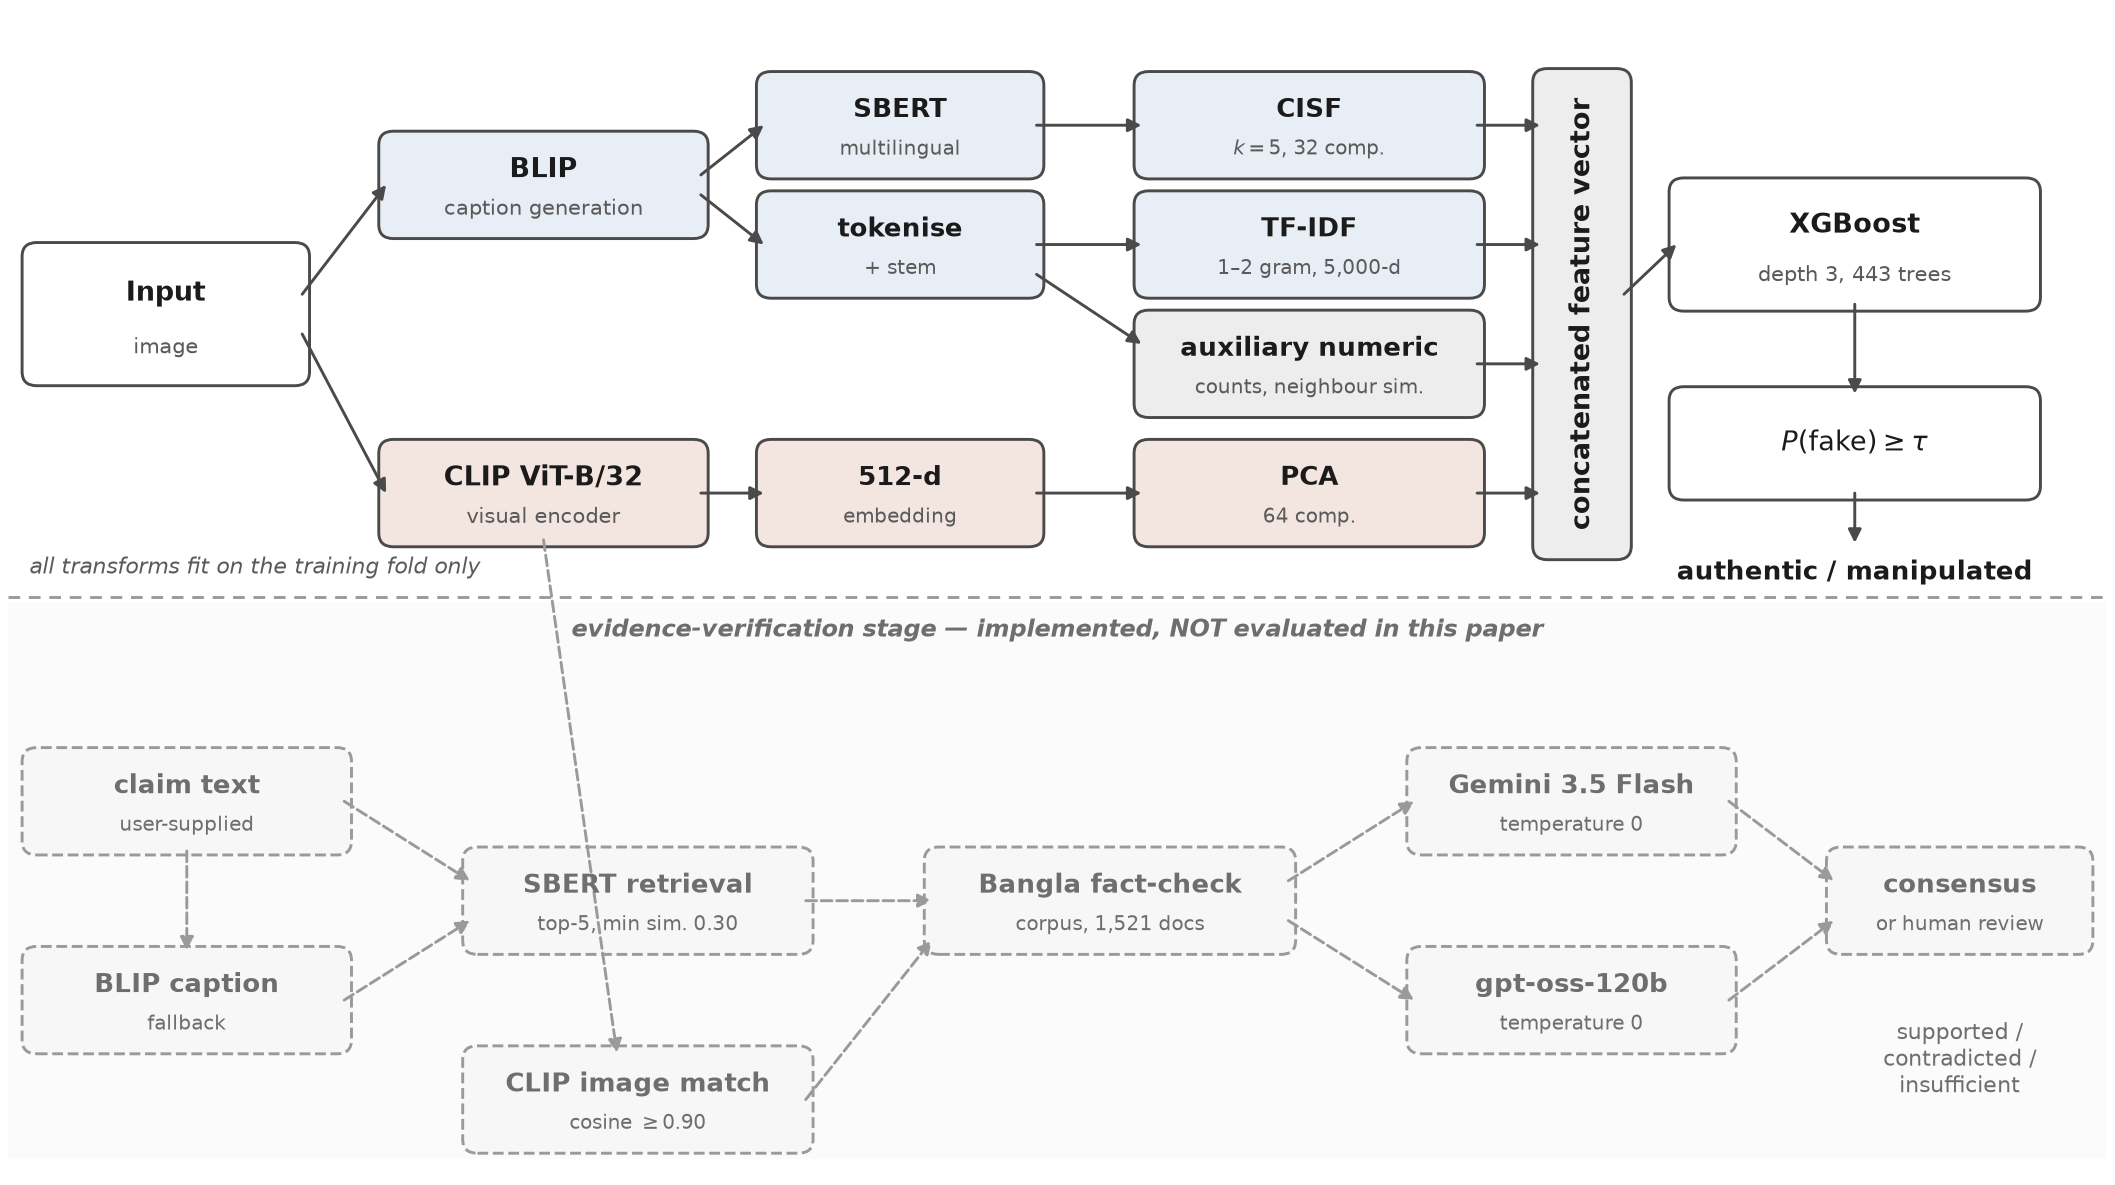
\includegraphics[width=0.80\textwidth]{fig1_system_architecture.png}
\caption{\sysname{} architecture. \textbf{Upper band (evaluated):} the four
feature blocks of Section~\ref{sec:features}, concatenated and classified by a
gradient-boosted tree; OCR is absent by design. \textbf{Lower band (dashed):}
the evidence-verification stage present in the implementation but not evaluated
here, and on which no result depends.}
\label{fig:arch}
\end{figure*}

\subsection{Benchmark and Attack Types}
\label{sec:data}

We use BanFakeMM \cite{banfakemm}, a detector-guided multimodal Bangla
benchmark built from 7{,}040 authentic news articles with images, drawn from
eight Bangla newspapers across eleven topical categories. The release provides
five adversarial sets---AdversarialEdit, AdversarialGen, LinguisticAttack,
RandomSwap and SemanticSwap---each containing 1{,}000 authentic and 1{,}000
manipulated samples, so every split is balanced by construction. Each record
carries an \texttt{article\_id}, a \texttt{source\_dataset} and a category, and
in the released master file 1{,}863 article identifiers carry both an authentic
image and its manipulated counterparts. Provenance is published, and we use it
rather than infer it (Section~\ref{sec:articles}).

Labels are deterministic: a sample is manipulated if the benchmark's
construction pipeline produced it, not if an annotator judged it so. That makes
the labels reproducible and the task well defined, but it also means a model
may learn to recognise the construction pipeline rather than the manipulation.
Section~\ref{sec:normalise} removes the part of that signature which lives
outside the image content; the part that survives resampling we cannot separate
from the manipulation itself, and we say so where it matters.

The classifier is trained on AdversarialEdit and evaluated under shift on
AdversarialGen. The three remaining splits manipulate article text and leave
the photograph untouched, which makes them undecidable for an image-only model
though presumably well posed for one that also reads the text;
Section~\ref{sec:detectable} demonstrates this rather than assuming it, and
reports what a model does on them.

\subsection{Image Normalisation}
\label{sec:normalise}

Before any feature is extracted, every image passes through one identical
re-encoding: resized to $384 \times 384$ with Lanczos resampling, converted to
RGB, saved as JPEG at quality 90, with no EXIF block carried over. Resolution,
aspect ratio, file format, colour mode and EXIF are therefore constant across
classes; image content is preserved.

This is not cosmetic. In AdversarialEdit all 1{,}000 manipulated images are
$1408 \times 768$ while the authentic images span many resolutions and formats,
and a classifier given only that metadata---no pixels at all---separates the
classes perfectly (Section~\ref{sec:artefact}). Without normalisation, any
reported accuracy is unidentifiable: it may be reading content, or it may be
reading the file header. We report the normalised figures as the primary
results and, where a comparison with the uncontrolled setting is informative,
give both and label them.

\subsection{Contamination Screening}
\label{sec:dedup}

\subsubsection{Image-level}
Filename comparison is not sufficient, since a manipulated image is an edited
copy of an authentic one and the two can carry unrelated names. Every image the
study uses is screened by content instead. Each is reduced to a 64-bit DCT
perceptual hash (pHash), a 64-bit difference hash (dHash) and its CLIP
embedding; a pair is a near-duplicate when either Hamming distance is at most
$2$ or the CLIP cosine similarity is at least $0.98$, and pairs are merged with
union-find. These thresholds sit in a clear gap: of 3.5 million candidate
pairs, 94 lie at pHash distance $0$ and only 102 at distance $6$ or below.
Duplicates are near-exact, and looser settings chain unrelated images into
implausible clusters.

Screening is applied in both directions that matter: within the training split,
to build cross-validation groups, and from every evaluation partition against
everything the models have seen---the base training set together with the
adaptation set.

\subsubsection{Article-level}
\label{sec:articles}
An image screen removes repeated pictures, not repeated stories: two different
photographs of the same event share entities, scene and caption vocabulary, and
different pixels do not rule that out. Because every image in this benchmark is
named by its source article, the check is exact rather than inferred---the
filename stem is the \texttt{article\_id} in each distributed set, which we
verified by content hash against the released master file.

We therefore report article-level overlap alongside the image-level screen
rather than folding one into the other, and we state the screening claim
accordingly: the pipeline removes image duplicates, and measures the residual
article overlap. Section~\ref{sec:articlescreen} gives the measured effect on
the conclusions.

\subsection{Partitioning}
\label{sec:partition}

AdversarialEdit supplies the training corpus: 2{,}000 images, which the
image-level screen resolves into 1{,}980 groups. Every fold in
Section~\ref{sec:ablation} is built with \texttt{StratifiedGroupKFold} over
those groups and asserted group-disjoint at run time.

AdversarialGen supplies the shift evaluation. Setting aside its distributed
80/10/10 partition, whose proportions do not suit a three-way adaptation study,
we repartition its 2{,}000 images at a fixed seed: 300 for supervised
adaptation, 150 for decision-threshold selection, 200 forming the sealed
partition used by earlier work on this system, and 1{,}350 held back entirely.
The adaptation and validation partitions are screened against the training set,
leaving 148 validation images; the adaptation partition keeps all 300, since a
duplicate inside training data is redundancy rather than leakage and pruning it
would confound the adaptation contrast with a change in training-set size.

The primary sealed partition is the block of 1{,}350 images, which entered no
training, tuning or threshold-selection step of any kind and had never been
scored. Screened against the base training set and the adaptation set under the
full criteria above---42 images removed, 21 by pHash, 40 by dHash and 24 by
CLIP cosine---it retains \textbf{1{,}308 images}, 658 of them manipulated. The
older 200-image block, which screening reduces to 194, has been scored before
and is therefore no longer pristine; we use it only where a direct comparison
with the earlier measurement is the point, and label it as such.

\subsection{Features and Classifier}
\label{sec:features}

A BLIP model generates a caption per image; OCR was evaluated during ablation
and removed (Section~\ref{sec:ablation}). The caption is tokenized and stemmed,
with separate handling for Bangla and Latin script, for TF-IDF features, and
separately encoded by multilingual SBERT. That embedding is refined through
CISF: combined with the weighted average of its $k=5$ nearest training
neighbours at fusion weight $\alpha=0.65$, re-normalized, and reduced to 32
principal components. A CLIP vision encoder
(\texttt{openai/clip-vit-base-patch32}) independently produces a
512-dimensional embedding, $L_2$-normalised and reduced to 64 components. These
were fixed design choices rather than outcomes of a search; a sensitivity study
over $k$ and $\alpha$, and comparison against adaptive fusion
\cite{mmfusionnet,claaf}, is left for future work.

The full vector concatenates four blocks, each fit only on the training fold:
the CISF caption embedding, the CLIP embedding, TF-IDF over the caption
($1$--$2$ grams, vocabulary capped at 5{,}000, minimum document frequency 3),
and auxiliary numeric features. Each training embedding's neighbour search
excludes itself, and at inference an unseen embedding is compared only against
this fixed training-set reference. Classification uses XGBoost
(\texttt{max\_depth}~3, \texttt{learning\_rate}~0.0742,
\texttt{n\_estimators}~443, \texttt{subsample}~0.866,
\texttt{colsample\_bytree}~0.683, \texttt{min\_child\_weight}~2,
\texttt{gamma}~0.143, \texttt{reg\_alpha}~$1.01\times10^{-5}$,
\texttt{reg\_lambda}~4.911), selected by randomized search over 8 sampled
configurations under 3-fold cross-validation.

\subsection{Protocol, Thresholds and Statistics}
\label{sec:training}

\subsubsection{Thresholds}
The operating threshold is selected on held-out validation data, never on an
evaluation partition, under a rule fixed before the sweep was run: $\tau$
maximizes fake-class F1 on the screened 148-image validation partition over a
$0.01$-step grid, ties broken by the median of the tied run. The sealed
partition is then scored once per threshold, after all training and threshold
decisions are frozen. Thresholds are selected separately for the normalised and
unnormalised settings, since the two produce differently calibrated scores, and
neither is reselected on test data.

Same-distribution figures are computed at the conventional $\tau = 0.50$
cut-off; no threshold search is performed on the training split, so those
numbers carry no selection effect.

\subsubsection{Cross-validation and dependence}
Ablation results come from repeated stratified 5-fold grouped cross-validation
over the clusters of Section~\ref{sec:dedup}---two repeats, ten folds---with
identical splits and fixed hyperparameters across every configuration and all
transforms fit inside the training fold only.

Repeated cross-validation does not yield independent observations: each image
is held out once per repeat, and any two training folds overlap in four fifths
of their rows. We therefore never stack repeats. Out-of-fold probabilities are
averaged across repeats so that each image contributes exactly one prediction
to any paired test, and fold-level comparisons use the Nadeau--Bengio corrected
resampled $t$ interval, which adds the train/test overlap ratio
($n_{\text{test}}/n_{\text{train}} = 0.25$ at five folds) to the naive $1/J$
variance term---a $3.5\times$ inflation here. The $\pm$ values reported beside
cross-validated accuracies are the spread across folds, not standard errors,
and no significance claim rests on them.

\subsubsection{Metrics and uncertainty}
Results are reported as accuracy, precision, recall and F1 for the manipulated
class, with authentic-class recall added under shift. Fake-recall is the more
safety-critical quantity---a missed manipulation circulates unchecked whereas a
false alarm costs only a review step---which is why the selection rule
maximizes fake-class F1.

For contrasts between two models on the same sealed partition we report AUROC
as the primary statistic. It is threshold-free, and the alternative---accuracy
at a fixed operating point---conflates a change in the model with a change in
where the cut-off happens to sit; Section~\ref{sec:adaptation} shows the two
disagreeing in sign on the same data. Confidence intervals on sealed-partition
quantities come from a paired bootstrap over images with $5{,}000$ resamples;
paired model comparisons additionally report an exact McNemar test over
discordant predictions.

\subsubsection{Seeds and reproducibility}
Every contrast on the sealed partition is run with eight seeds
($42$, $101$, $202$, $303$, $404$, $505$, $606$, $707$), varying fold
assignment, the PCA transforms and the classifier together; we report the
seed-averaged statistic and the seed-to-seed standard deviation, so that the
size of an effect can be read against the variability of the procedure that
produced it. Single-seed results are reported nowhere except where we compare
against an earlier single-seed measurement. All manifests, per-image
probabilities, screening clusters and the full validation sweeps are released
with the code.


%==============================================================
% RESULTS SECTION -- journal version.
%
% Every number below is traceable to a file in the project root:
%   ablation rows              ablation_grouped_summary.csv
%   metadata / artefact rows   artefact_control.csv
%   per-split ceilings         split_ceilings.csv
%   text-split performance     textsplit_results.csv, textsplit_proof.csv
%   shift, n=194 controlled    shift_controlled_results.csv
%   shift, n=1308 both ways    big_sealed_results_v2.csv
%   adaptation, 8 seeds        adaptation_final.csv, adaptation_final_seeds.csv
%   article-level screen       article_screen.csv
%
% This section SUPERSEDES the conference version's Section IV-C retraction.
% That retraction rested on an accuracy comparison at one threshold, on 194
% images, with one seed. Subsection E explains what a better measurement says.
%==============================================================

\section{Experimental Results}

\subsection{Per-Modality Ablation}
\label{sec:ablation}

Table~\ref{tab:ablation} reports every configuration under one protocol:
repeated stratified 5-fold \emph{grouped} cross-validation over the
near-duplicate clusters of Section~\ref{sec:dedup}, two repeats, identical
splits and hyperparameters throughout, every transform fit inside the training
fold only, and all figures taken at the conventional $\tau = 0.50$ cut-off.

OCR in isolation reaches $57.35$ percent with a fake-recall of $33.85$. That is
above the 50 percent chance baseline---about three fold-standard-deviations
above it---so the modality is not devoid of signal; but it recovers only a
third of the manipulated class, and adds nothing once CLIP is present. We
remove it, and we do not generalize the result beyond this benchmark:
MultiBanFakeDetect \cite{multibanfake} indicates text-in-image remains a
meaningful vector for Bangla misinformation, and on a corpus where
manipulation is carried by embedded text the ordering could invert.

Every text-only configuration saturates below 78 percent while every
configuration containing CLIP exceeds 95. The gap is not subtle, and
Section~\ref{sec:detectable} explains it: in this split the manipulation is
applied to the pixels and to nothing else.

The comparison that matters for placing this work is against
MultiBanFakeDetect \cite{multibanfake}, the closest prior system in language
and modality scope. We run its feature families---a DenseNet-169 visual
backbone, and that backbone fused with an mBERT text branch---through the
identical pipeline: same folds, same PCA reduction, same classifier, same
cut-off, so that only the backbone differs. DenseNet-169 reaches
$89.28 \pm 1.48$ percent against CLIP's $95.38 \pm 1.33$, a gap of $6.10$
points; with the artefact removed the gap is $6.13$. Adding the mBERT branch
moves DenseNet to $89.65$, which leaves it $5.73$ points behind CLIP alone.

Two things in that comparison are worth separating. The first is the margin
itself, which is large and stable across both encodings, and which we would
expect from a backbone trained contrastively on image--text pairs against one
trained for ImageNet classification. The second is more informative: the mBERT
branch contributes $+0.37$ points to DenseNet, and $+0.45$ with the artefact
removed---the same near-zero contribution the caption pathway makes to CLIP in
Section~\ref{sec:fusion}. Two independently chosen visual backbones give the
same verdict on the text branch, which makes that verdict a property of the
task rather than a quirk of our feature choice.

What this comparison is not is a reimplementation of MultiBanFakeDetect as
published. That system reads the article's own title and body, which our
pipeline never takes as input, so its text branch here encodes the BLIP caption
instead. The comparison therefore isolates the backbone and the fusion
structure under one protocol; it does not establish how the published system
would perform with the inputs it was designed for.

No row is marked best among the four CLIP-containing configurations. Their
total spread is $0.17$ points against a per-fold standard deviation of
$1.0$--$1.4$, and the ordering reverses under an unrelated methodological
change---ungrouped folds put CLIP-only ahead by $0.18$ points, duplicate-aware
folds put the fused configuration ahead by $0.02$. Accuracy does not decide
between them; Section~\ref{sec:fusion} decides on other grounds.

\begin{table}[!tb]
\caption{Baselines, Per-Modality Ablation and the Artefact Control Under One
Protocol: Repeated Stratified 5-Fold \emph{Grouped} Cross-Validation Over
Near-Duplicate Clusters ($2$ Repeats, $10$ Folds), in Percent.}
\label{tab:ablation}
\centering
\setlength{\tabcolsep}{3.5pt}
\footnotesize
\begin{tabular}{lcccc}
\toprule
\textbf{Configuration} & \textbf{Acc.} & \textbf{Prec.$_{f}$} &
\textbf{Rec.$_{f}$} & \textbf{F1$_{f}$} \\
\midrule
\multicolumn{5}{l}{\emph{Reference baselines}} \\
Metadata only (no pixels)$^{\ddagger}$ & 100.00 $\pm$ 0.00 & 100.00 & 100.00 & 100.00 \\
Linear SVM (TF-IDF)     & 73.93 $\pm$ 1.35 & 72.42 & 77.40 & 74.80 \\
XGBoost (TF-IDF + num.) & 77.15 $\pm$ 1.86 & 77.50 & 76.60 & 77.00 \\
DenseNet-169$^{\S}$     & 89.28 $\pm$ 1.48 & 89.10 & 89.50 & 89.30 \\
\quad artefact-controlled & 88.22 $\pm$ 1.57 & 88.49 & 87.90 & 88.19 \\
DenseNet-169 + mBERT$^{\S}$ & 89.65 $\pm$ 1.50 & 89.39 & 90.00 & 89.68 \\
\quad artefact-controlled & 88.67 $\pm$ 1.97 & 88.71 & 88.65 & 88.66 \\
\midrule
\multicolumn{5}{l}{\emph{Modality ablation}} \\
OCR only              & 57.35 $\pm$ 2.34 & 63.97 & 33.85 & 44.22 \\
Caption only          & 74.50 $\pm$ 2.68 & 75.22 & 73.25 & 74.16 \\
Text only             & 76.05 $\pm$ 1.82 & 76.42 & 75.45 & 75.87 \\
Text + CISF           & 77.38 $\pm$ 2.10 & 77.41 & 77.55 & 77.40 \\
\midrule
CLIP only$^{\dagger}$ & 95.38 $\pm$ 1.33 & 94.68 & 96.15 & 95.41 \\
\quad on artefact-controlled images & 94.35 $\pm$ 0.94 & 94.17 & 94.60 & 94.37 \\
Text + CLIP           & 95.28 $\pm$ 1.04 & 95.04 & 95.55 & 95.28 \\
CLIP + CISF           & 95.23 $\pm$ 1.38 & 95.07 & 95.40 & 95.23 \\
Caption + CISF + CLIP & 95.40 $\pm$ 1.09 & 95.13 & 95.70 & 95.41 \\
\bottomrule
\end{tabular}
\par\smallskip\parbox{\linewidth}{\footnotesize \footnotesize Subscript $f$ denotes the
manipulated class; $\pm$ is the spread across folds, not a standard error.
$^{\dagger}$ the selected configuration, on the grounds of
Section~\ref{sec:fusion}. $^{\ddagger}$ width, height, area, aspect ratio, file
size, format and colour mode only, with no image content---see
Section~\ref{sec:artefact}. $^{\S}$ the feature families of
MultiBanFakeDetect \cite{multibanfake} run through this protocol; see the text
for what that comparison does and does not establish.}
\end{table}

\subsection{Does the Caption Pathway Contribute?}
\label{sec:fusion}

Accuracy parity does not settle whether the caption pathway is worth keeping: a
feature block can leave accuracy unchanged yet still improve ranking or
calibration, neither of which is visible in Table~\ref{tab:ablation}. We
compare CLIP-only against the fused configuration on four measures in both
regimes, everything else held fixed.

\begin{table}[!tb]
\caption{CLIP-Only Versus the Fused Configuration, Same Hyperparameters and
Folds. AUROC and Brier Are Threshold-Independent; ECE Uses $10$ Bins. Arrows
Mark the Preferred Direction.}
\label{tab:fusion}
\centering
\setlength{\tabcolsep}{4pt}
\footnotesize
\begin{tabular}{llcccc}
\toprule
& \textbf{Model} & \textbf{Acc.}$\uparrow$ & \textbf{AUROC}$\uparrow$ &
\textbf{Brier}$\downarrow$ & \textbf{ECE}$\downarrow$ \\
\midrule
\multirow{2}{*}{same-d.}
& CLIP only & 95.38 & 0.9918 & 0.0349 & 3.17 \\
& Fused     & 95.40 & 0.9920 & 0.0342 & 3.05 \\
\midrule
\multirow{2}{*}{shift}
& CLIP only & 85.05 & \textbf{0.9759} & \textbf{0.0936} & \textbf{4.06} \\
& Fused     & 85.57 & 0.9732 & 0.1076 & 7.31 \\
\bottomrule
\end{tabular}
\par\smallskip\parbox{\linewidth}{\footnotesize \footnotesize Same-distribution figures
are pooled out-of-fold values over the folds of Table~\ref{tab:ablation};
shift figures are the 194-image partition at $\tau = 0.50$, so both models meet
the same operating point. That partition is easier than the full sealed set:
CLIP-only reaches AUROC $0.976$ on it and $0.941$ on the 1{,}308-image partition
(Fig.~\ref{fig:roc}), so the shift rows support the paired comparison between the
two models, not an absolute level. Both regimes use the original files: see the
caveat at the end of this subsection.}
\end{table}

Same-distribution, the two are indistinguishable on every measure. The paired
fold-level differences (fused minus CLIP-only), with the Nadeau--Bengio
correction for fold dependence \cite{nadeau}, are $+0.03$ accuracy points
(95\% CI $[-0.98, +1.03]$, $p = 0.956$), $+0.0002$ AUROC ($p = 0.811$),
$-0.0006$ Brier ($p = 0.709$) and $-0.12$ ECE points ($p = 0.794$); McNemar on
the repeat-averaged out-of-fold predictions, one per image, finds 21 images the
fused model alone classifies correctly against 20 for CLIP-only (exact
$p = 1.000$). Every interval spans zero, and the uncorrected intervals---which
we do not report---were $1.9\times$ narrower.

Under shift the comparison turns against the caption pathway. Its
$+0.5$-point accuracy advantage sits well inside its interval
($[-2.6, +3.6]$), while its calibration is clearly worse: Brier rises from
$0.0936$ to $0.1076$ and expected calibration error from $4.06$ to $7.31$
points---least trustworthy exactly where the threshold has to be chosen. The
pathway costs a BLIP forward pass, an SBERT encoding and a nearest-neighbour
search per image and returns nothing measurable, so we do not claim it as a
contribution and adopt CLIP-only as the recommended configuration.

We repeated the same-distribution comparison under the artefact control of
Section~\ref{sec:artefact}, regenerating the BLIP captions from the re-encoded
images, since the caption pathway reads the image and could carry the artefact
too. With every input taken from the re-encoded files, CLIP-only reaches
$94.35 \pm 0.99$ percent and the fused configuration $94.68 \pm 1.07$: a
difference of $+0.33$ points (Nadeau--Bengio 95 percent CI $[-0.51, +1.16]$),
$-0.0007$ AUROC ($[-0.0023, +0.0008]$), and no difference in Brier score or
expected calibration error; the out-of-fold McNemar test splits $19$ to $17$
($p = 0.87$). The verdict is unchanged. What we did not repeat is the
distribution-shift comparison above, whose calibration gap was measured on the
original files, so that part remains uncontrolled.

\subsection{Dataset Artefacts and What Survives Them}
\label{sec:artefact}

An accuracy above 95 percent on a constructed benchmark deserves suspicion
before it deserves interpretation. In the AdversarialEdit split every one of
the 1{,}000 manipulated images is $1408 \times 768$, while the authentic images
are spread across many resolutions, formats and colour modes; AdversarialGen
carries the same signature in 995 of its 1{,}000 manipulated images. The
classes are separable without reading a single pixel, and the first row of
Table~\ref{tab:ablation} confirms it: a classifier given only width, height,
area, aspect ratio, file size, format and colour mode reaches
$100.00 \pm 0.00$ percent under the same grouped protocol.
Figure~\ref{fig:resolution} shows the fingerprint: the manipulated class sits in
a single column, and the authentic class, spread over 196 distinct sizes in
AdversarialEdit and 157 in AdversarialGen, never uses it.

\begin{figure}[!tb]
\centering
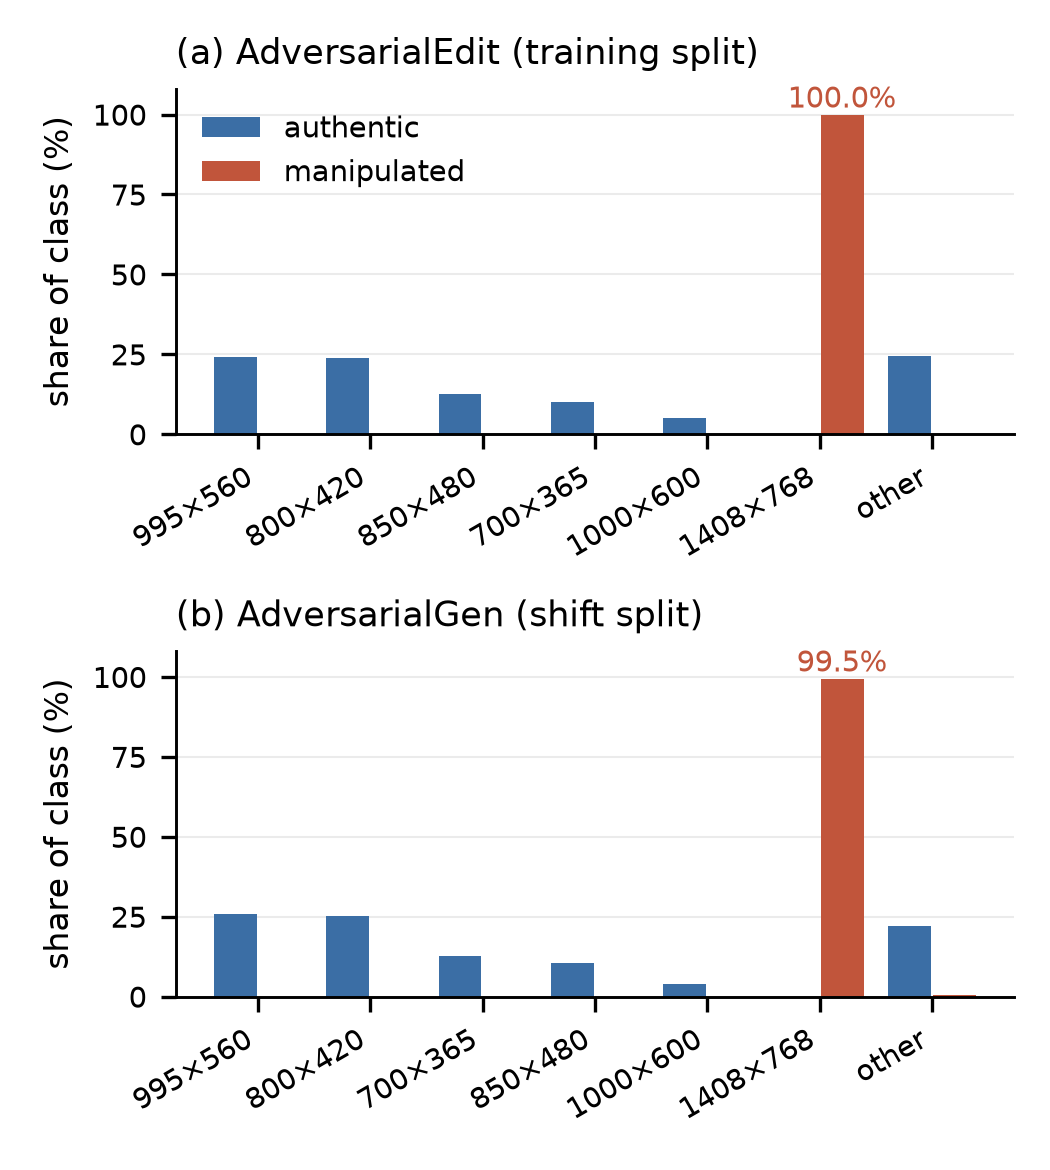
\includegraphics[width=\columnwidth]{fig_j_resolution.png}
\caption{Resolution fingerprint in the two image-attack splits. Manipulated
images are $1408 \times 768$ in $100.0$ percent (a) and $99.5$ percent (b) of
cases; authentic images are spread over many sizes, none of them $1408 \times
768$. Bars show the share of each class at its five most common sizes, plus the
manipulated class's modal size.}
\label{fig:resolution}
\end{figure}

We therefore re-encode every image through one identical pipeline before
feature extraction---resized to $384 \times 384$, converted to RGB, saved as
JPEG at quality 90, EXIF discarded---so that resolution, aspect ratio, format,
colour mode and EXIF are destroyed while content is preserved. Repeating the
CLIP-only configuration on the re-encoded corpus, with the same folds,
hyperparameters and cut-off, gives $94.35 \pm 0.94$ percent against
$95.38 \pm 1.33$ on the originals: a loss of $1.03$ points. The discriminative
signal is in the pixels, not in the storage fingerprint.

The shortcut is not a property of the corpus as a whole, and the benchmark
contains its own control. Table~\ref{tab:shortcut} applies the same
metadata-only classifier to all five adversarial splits. It separates the
classes perfectly in exactly the two splits whose manipulated images are
produced by an image pipeline, and finds nothing in the three that rewrite the
article text and reuse the photograph: AUROC $1.0000$ against $0.3175$ to
$0.4892$. The shortcut therefore tracks the attack type rather than the
benchmark, which is what one would expect if it originates in a generator
emitting at a fixed resolution.

\begin{table}[!tb]
\caption{Metadata-Only Classifier Across All Five Adversarial Splits, Same
Feature Set as Table~\ref{tab:ablation}, 5-Fold Cross-Validation. No Pixel
Content Is Used.}
\label{tab:shortcut}
\centering
\setlength{\tabcolsep}{4pt}
\footnotesize
\begin{tabular}{llcc}
\toprule
\textbf{Split} & \textbf{Manipulation} & \textbf{Acc.} & \textbf{AUROC} \\
\midrule
AdversarialEdit  & image & 100.00 $\pm$ 0.00 & 1.0000 \\
AdversarialGen   & image & 99.35 $\pm$ 1.30 & 1.0000 \\
\midrule
LinguisticAttack & text  & 48.95 $\pm$ 1.61 & 0.4892 \\
RandomSwap       & text  & 39.05 $\pm$ 3.87 & 0.3318 \\
SemanticSwap     & text  & 37.05 $\pm$ 1.54 & 0.3175 \\
\midrule
MultiBanFakeDetect$^{\ddagger}$ & fake-labelled & 77.51 $\pm$ 4.55 & 0.8533 \\
\bottomrule
\end{tabular}
\par\smallskip\parbox{\linewidth}{\footnotesize \footnotesize Values below chance mean the
metadata carries no usable signal and is, if anything, mildly misleading---
consistent with the image reuse across labels documented in
Section~\ref{sec:detectable}. $^{\ddagger}$A second corpus
\cite{multibanfake}: 9{,}597 images, label read from the file name, same
metadata features, plain 5-fold cross-validation.}
\end{table}

Two limits on what this establishes. Re-encoding removes the storage artefact,
not a generation-pipeline signature that survives resampling. If every
manipulated image carries the same synthesis fingerprint, a visual model may be
recognising the generator rather than the manipulation---and because BanFakeMM
defines its labels by the construction pipeline, the two are difficult to
separate even in principle. We report the controlled figure throughout and
flag, in each table, which numbers are controlled and which are not.

The control of Table~\ref{tab:shortcut} is internal to one benchmark, so we ran
the same file-metadata classifier on a second Bangla multimodal corpus,
MultiBanFakeDetect \cite{multibanfake}: 9{,}600 images, half labelled fake,
with the label read from the file name. The artefact is present there but far
weaker than in BanFakeMM. Metadata alone reaches $77.5$ percent accuracy
(AUROC $0.853$) under plain five-fold cross-validation, $82.8$ percent
(AUROC $0.902$) with byte-identical files grouped, and $77.1$ percent
(AUROC $0.852$) when trained on the official Train folder and scored on Test,
against $100$ percent in BanFakeMM's image-attack splits and $50$ percent at
chance. One size, $728\times410$, accounts for $39.5$ percent of the
fake-labelled images and for at most $7.2$ percent of any size among the
authentic ones, and $85$ files occur under both labels. We therefore read the
shortcut as a property of constructed Bangla benchmarks that varies in
strength, not as a feature of BanFakeMM alone. Whether the fake-labelled images
in that corpus are manipulated or merely sourced differently we did not
verify, and we use ``fake-labelled'' for that reason.

\subsection{Which Attack Types Are Detectable From Pixels}
\label{sec:detectable}

BanFakeMM provides five adversarial splits. They are not five variations on
one task. We checked each manipulated image against the benchmark's full
authentic corpus (the 7{,}040 real images of the released master file) by
content hash and by perceptual hash; Table~\ref{tab:ceiling} reports the
result.

In AdversarialEdit and AdversarialGen not one manipulated image reproduces an
authentic one. In LinguisticAttack, RandomSwap and SemanticSwap \emph{every}
manipulated image is byte-identical to an authentic image---1{,}000 of 1{,}000,
at perceptual-hash distance zero. Those attacks alter the article text and
leave the photograph untouched. An image-only classifier cannot exceed chance
on them, not because it is weak but because the label is not a function of its
input.

\begin{table}[!tb]
\caption{Per-Split Image-Only Ceiling and Measured Performance. The Ceiling Is
$1$ Minus the Share of Manipulated Images That Reproduce an Authentic Image.
Measured Figures Are the Zero-Shot CLIP-Only Model at $\tau = 0.50$.}
\label{tab:ceiling}
\centering
\setlength{\tabcolsep}{4pt}
\footnotesize
\begin{tabular}{lccccc}
\toprule
\textbf{Split} & \textbf{Manip.} & \textbf{Reproduced} &
\textbf{Ceiling} & \textbf{Acc.} & \textbf{AUROC} \\
\midrule
AdversarialEdit  & 1000 & 0    & 100\% & --- & --- \\
AdversarialGen   & 1000 & 0    & 100\% & 85.1 & --- \\
\midrule
LinguisticAttack & 1000 & 1000 & 0\%   & 49.5 & 0.4832 \\
RandomSwap       & 1000 & 1000 & 0\%   & 50.5 & 0.5165 \\
SemanticSwap     & 1000 & 1000 & 0\%   & 50.5 & 0.5094 \\
\bottomrule
\end{tabular}
\par\smallskip\parbox{\linewidth}{\footnotesize \footnotesize ``Reproduced'' counts
manipulated images byte-identical to an authentic image in the benchmark's
master file; all of them are also at perceptual-hash distance $0$.
AdversarialEdit is the training split, so no held-out figure is quoted.}
\end{table}

The measured numbers match the prediction exactly. Accuracy on the three
text-attack splits is $49.5$, $50.5$ and $50.5$ percent, and AUROC is
$0.4832$, $0.5165$ and $0.5094$---indistinguishable from a coin, and
threshold-independent, so no operating point can rescue them. The signature is
visible in the structure as well: fake-recall and real-recall sum to almost
exactly 100 at every threshold we tried, which is what happens when lowering a
cut-off moves images out of one class and into the other at the same rate in
both. Figure~\ref{fig:roc} puts the contrast in one picture: on the
image-attack split the ROC curve climbs steeply, and on the three text-attack
splits it lies on the diagonal.

\begin{figure}[!tb]
\centering
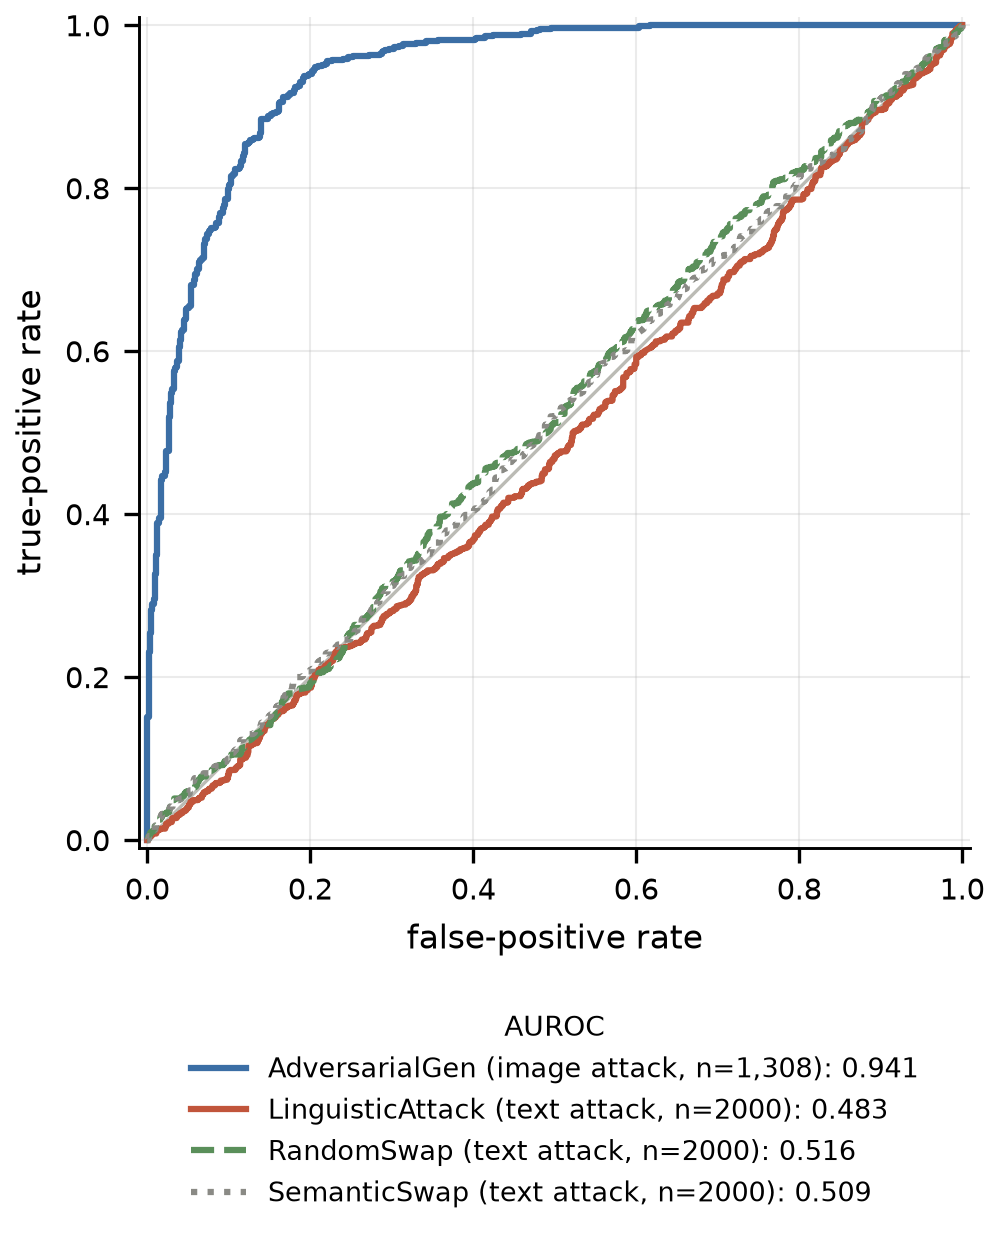
\includegraphics[width=0.95\columnwidth]{fig_j_roc.png}
\caption{ROC curves of the zero-shot CLIP-only model (seed 42, original files)
on the image-attack AdversarialGen split (the 1{,}308-image sealed partition)
and on the three text-attack splits (2{,}000 images each). The text-attack
curves are indistinguishable from chance because every manipulated image in
those splits is byte-identical to an authentic one.}
\label{fig:roc}
\end{figure}

Two further checks confirm the mechanism rather than merely the outcome. Where
a split's manipulated image is the same file as one of its own authentic
images---26, 38 and 131 such pairs respectively---the model assigns the two
\emph{exactly} the same probability, maximum absolute difference
$0.00\mathrm{e}{+}00$. And the mean predicted probability of the manipulated
class ($0.0703$, $0.0678$, $0.0808$) is within noise of the authentic class
($0.0790$, $0.0616$, $0.0739$). The 50 percent is arithmetic, not a deficiency.

The consequence for this paper is a scope statement rather than a result: our
system is image-derived end to end---BLIP caption, OCR and CLIP all read the
image, and the article's own text is never an input---so it is well posed on
two of the five splits and we evaluate it on those two only. The consequence
for the field is sharper: any image-level result reported across all five
BanFakeMM splits is averaging over three conditions in which the task is
undefined.

\subsection{Performance Under Distribution Shift}
\label{sec:shift}

Shift is measured from AdversarialEdit to AdversarialGen, the two splits
Section~\ref{sec:detectable} shows to be well posed. Thresholds are selected on
the disjoint 148-image validation partition under the rule fixed in
Section~\ref{sec:training} and are not reselected afterwards; the sealed
partition is scored once per threshold.

We enlarge the sealed partition well beyond the conference version. The 1{,}350
AdversarialGen images the study had never touched---not training, not
adaptation, not threshold selection---are screened against everything the
models have seen (base training plus the adaptation set) under the full
criteria of Section~\ref{sec:dedup}: perceptual-hash distance at most 2 on
either hash, or CLIP cosine at least $0.98$. That removes 42 images
(21 by pHash, 40 by dHash, 24 by CLIP cosine; 42 in union) and leaves
\textbf{1{,}308 sealed images}, 658 of them manipulated---$6.7\times$ the
194-image partition the conference version used.

\begin{table}[!tb]
\caption{Distribution Shift on the 1{,}308-Image Sealed Partition, Scored Once
Per Threshold, With and Without the Artefact Control. All Values in Percent.}
\label{tab:shift}
\centering
\setlength{\tabcolsep}{3pt}
\footnotesize
\begin{tabular}{llccccc}
\toprule
& \textbf{Setting} & \textbf{$\tau$} & \textbf{Acc.} &
\textbf{Prec.$_{f}$} & \textbf{Rec.$_{f}$} & \textbf{Rec.$_{r}$} \\
\midrule
\multirow{2}{*}{raw}
& Zero-shot & 0.09 & 87.2 & 83.1 & 93.5 & 80.8 \\
& Adapted   & 0.12 & 87.8 & 82.0 & 97.1 & 78.5 \\
\midrule
\multirow{2}{*}{ctrl.}
& Zero-shot & 0.25 & 84.9 & 86.6 & 82.7 & 87.1 \\
& Adapted   & 0.35 & 88.7 & 89.1 & 88.3 & 89.1 \\
\bottomrule
\end{tabular}
\par\smallskip\parbox{\linewidth}{\footnotesize \footnotesize ``raw'' uses the original
files and carries the artefact of Section~\ref{sec:artefact}; ``ctrl.'' uses
re-encoded images. Bootstrap 95\% CIs on accuracy (5{,}000 resamples), in row
order: $[85.3, 88.9]$, $[86.0, 89.6]$, $[82.9, 86.9]$, $[86.9, 90.4]$.}
\end{table}

Two things change under the control, and both matter. The selected thresholds
move from $0.09$ and $0.12$ to $0.25$ and $0.35$: on re-encoded images the
model is far better calibrated and no longer needs an extreme cut-off. And the
apparent benefit of thresholding collapses. On the 194-image partition,
re-encoded, moving from the default cut-off to the validation-selected one
bought $+0.5$ points ($87.6 \rightarrow 88.1$, 95 percent CI
$[-3.6, +4.6]$, McNemar $p = 1.000$), where the uncontrolled measurement had
suggested $+6.1$. \emph{We therefore withdraw the claim, made in the
conference version of this work, that almost the entire shift penalty is a
calibration effect.} It was largely an artefact of the uncontrolled encoding.

\subsection{Does Supervised Adaptation Help?}
\label{sec:adaptation}

The conference version of this work retracted a previously claimed adaptation
gain, on the basis that 300 additional target-style images changed sealed-test
accuracy by $-1.5$ points (95 percent CI $[-4.6, +1.5]$ as reported there; a
bootstrap run to convergence on the same per-image scores gives
$[-5.2, +1.5]$, which is the interval drawn in Fig.~\ref{fig:adaptation}). That
measurement was an accuracy comparison at one fixed threshold, on 194 images,
from a single model fit. It is the most fragile way to measure this effect, and
Table~\ref{tab:adaptation} and Fig.~\ref{fig:adaptation} show it was measuring
the wrong thing.

\begin{table}[!tb]
\caption{Effect of Supervised Adaptation on the 1{,}308-Image Sealed
Partition, Averaged Over Eight Seeds. $\Delta$AUROC Is Threshold-Free; CIs Are
Paired Bootstraps Over Images ($5{,}000$ Resamples).}
\label{tab:adaptation}
\centering
\setlength{\tabcolsep}{4pt}
\footnotesize
\begin{tabular}{lccccc}
\toprule
\textbf{Setting} & \textbf{AUROC$_{0}$} & \textbf{AUROC$_{a}$} &
\textbf{$\Delta$AUROC} & \textbf{95\% CI} & \textbf{$\Delta$Acc.} \\
\midrule
Raw        & 0.9422 & 0.9661 & $+0.0240$ & $[+0.0173, +0.0308]$ & $+1.40 \pm 0.69$ \\
Controlled & 0.9380 & 0.9652 & $+0.0273$ & $[+0.0205, +0.0344]$ & $+4.04 \pm 0.43$ \\
\midrule
\multicolumn{6}{l}{\emph{Article-disjoint subset ($n = 1{,}222$)}} \\
Raw        & 0.9432 & 0.9660 & $+0.0228$ & $[+0.0160, +0.0301]$ & $+1.61 \pm 0.76$ \\
Controlled & 0.9386 & 0.9655 & $+0.0270$ & $[+0.0202, +0.0343]$ & $+4.15 \pm 0.52$ \\
\bottomrule
\end{tabular}
\par\smallskip\parbox{\linewidth}{\footnotesize \footnotesize Subscripts $0$ and $a$
denote the zero-shot and adapted models. $\Delta$Acc. is at the fixed
validation-selected thresholds of Table~\ref{tab:shift}, reported as mean
$\pm$ standard deviation across seeds. Seed-to-seed standard deviation of
$\Delta$AUROC is $0.0018$ (raw) and $0.0017$ (controlled). All four rows use the
same eight seeds, the same training-row order and the same definition of
$\Delta$Acc.}
\end{table}

\begin{figure*}[!tb]
\centering
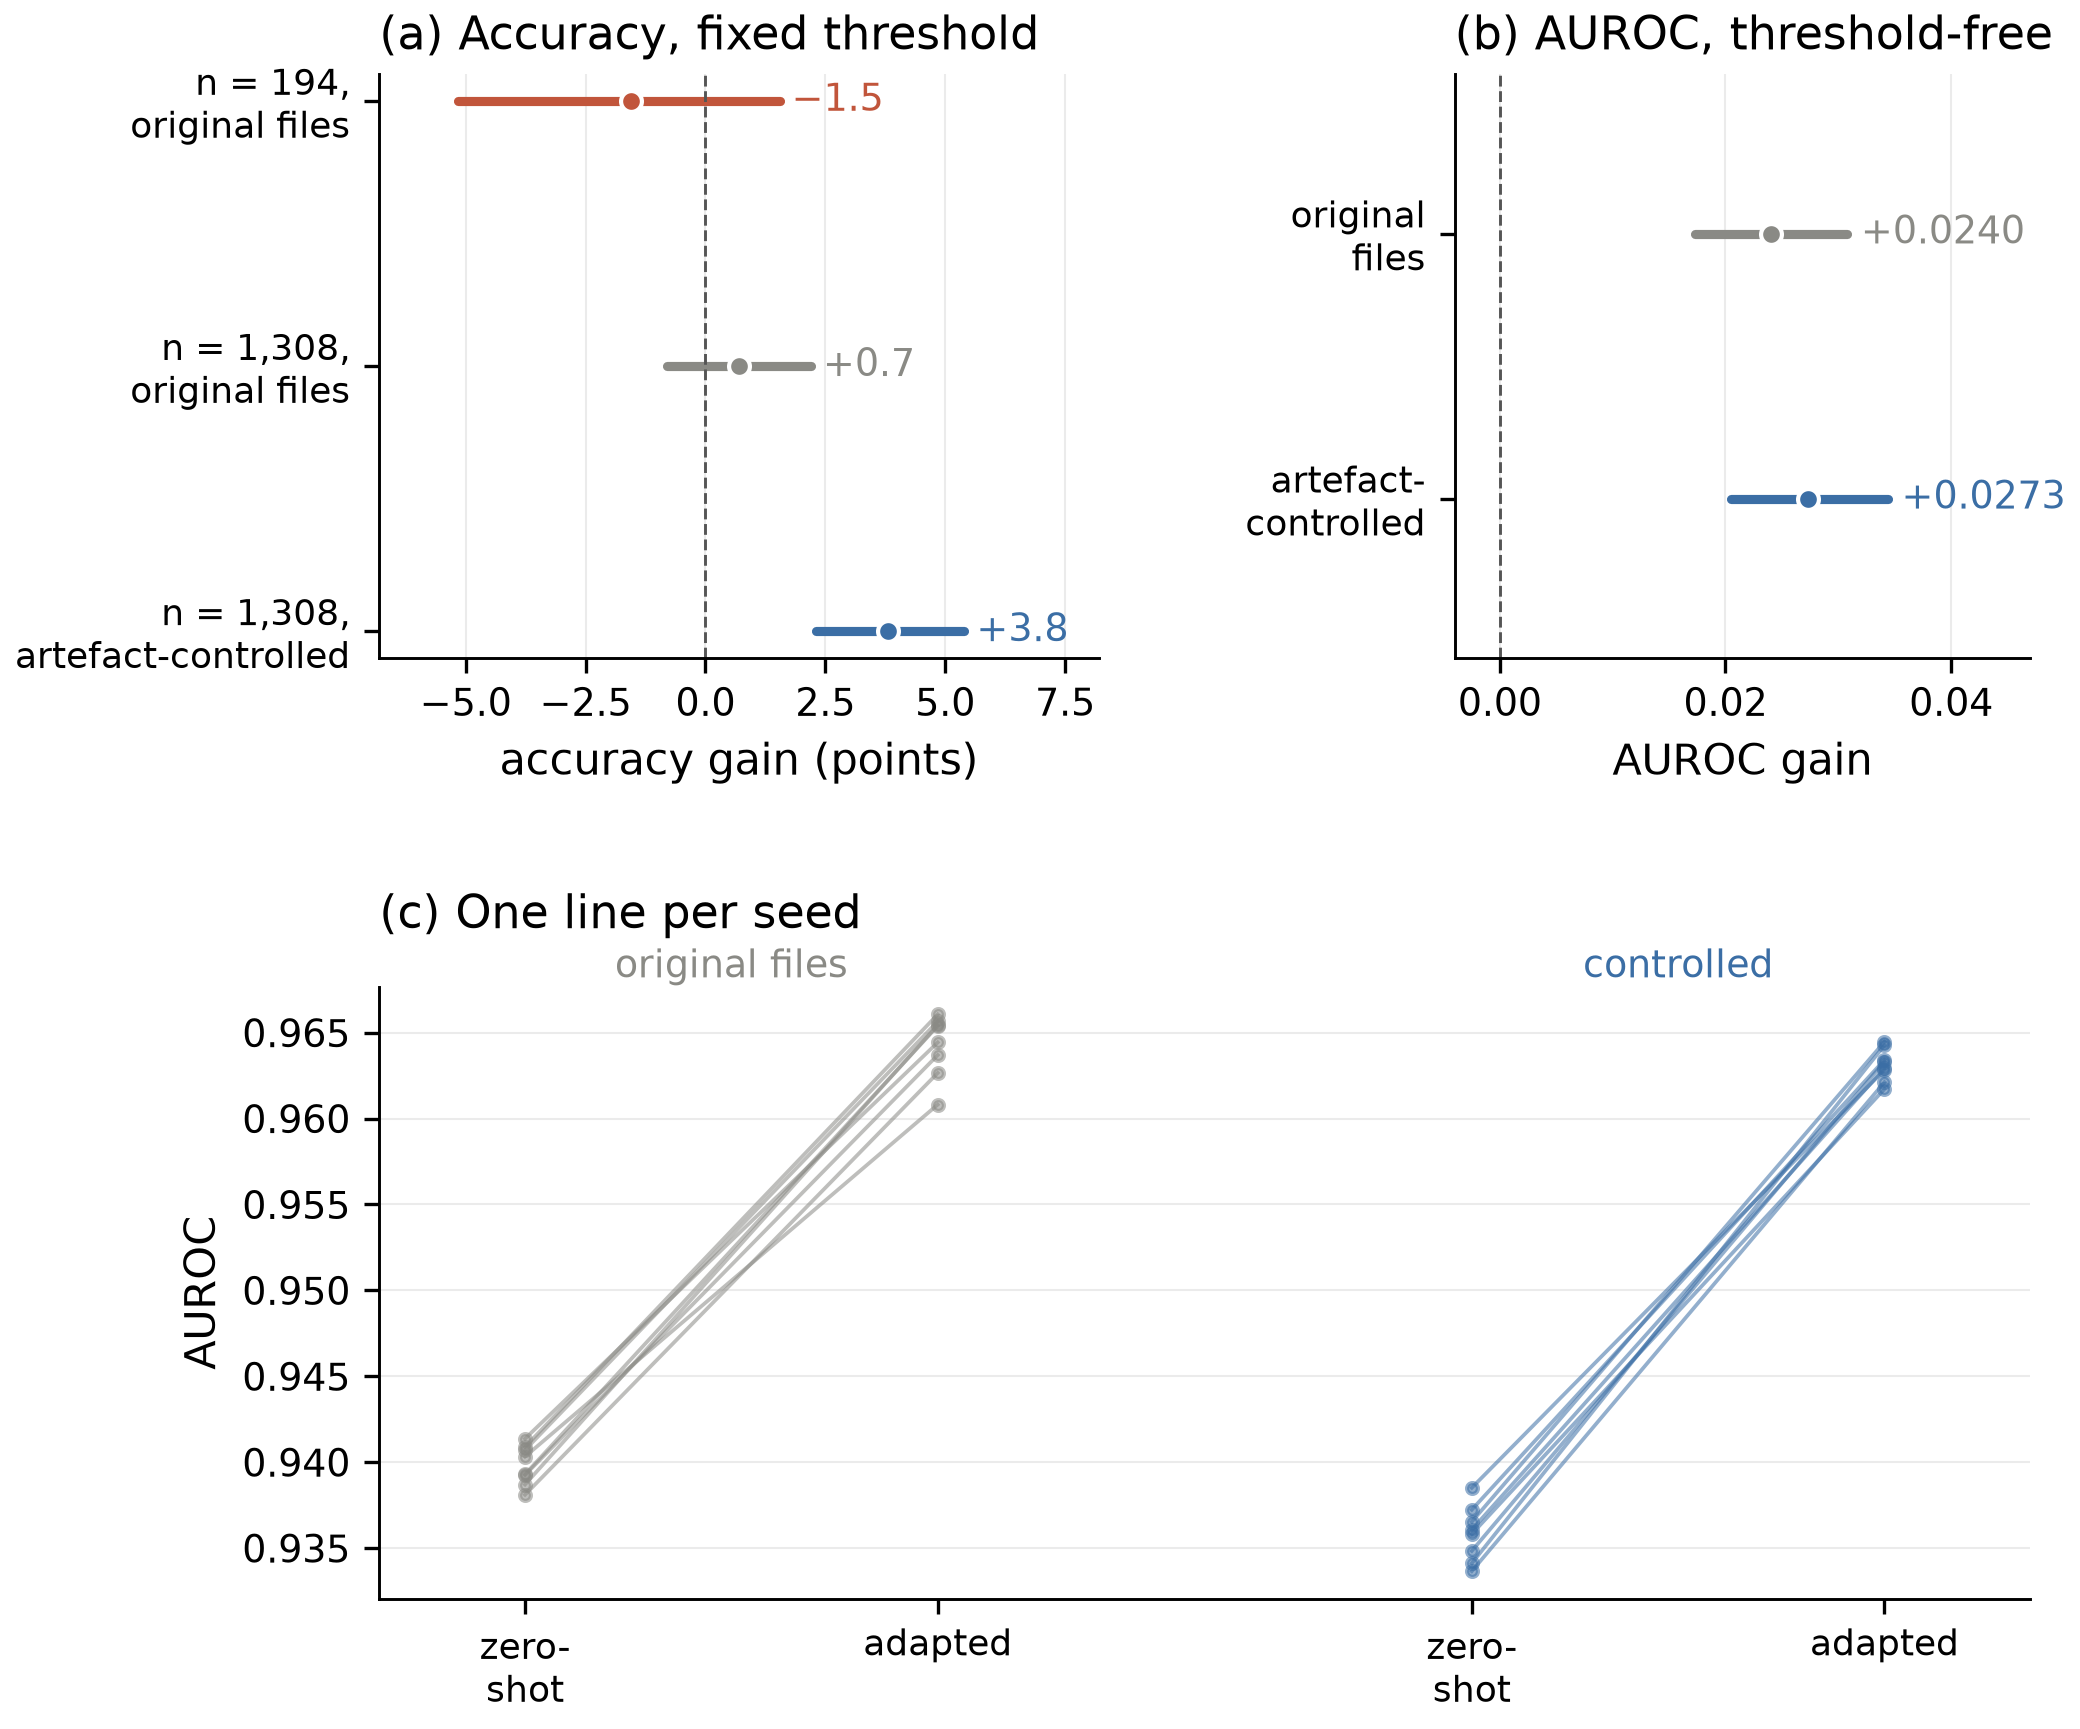
\includegraphics[width=0.82\textwidth]{fig_j_adaptation_springer.png}
\caption{The same intervention measured four ways. (a) Accuracy gain from
adaptation at a fixed threshold, each bar a single fit (seed 42) with a 95
percent bootstrap interval over images: it is negative on the 194-image
partition, indistinguishable from zero on 1{,}308 original files, and positive
on 1{,}308 artefact-controlled images; the eight-seed means are in
Table~\ref{tab:adaptation}. (b) The
threshold-free AUROC gain, with 95 percent intervals, is positive and similar in
both settings. (c) Per-seed AUROC before and after adaptation: it improves in
all 16 runs (eight seeds, two settings).}
\label{fig:adaptation}
\end{figure*}

Measured threshold-free, supervised adaptation improves the ranking by
$+0.0240$ AUROC on the original files and $+0.0273$ on re-encoded ones. Both
confidence intervals exclude zero by a wide margin, and the seed-to-seed
standard deviation---$0.0018$ and $0.0017$---is roughly one fourteenth of the
effect. The result does not depend on the artefact control: it is present, at
almost the same size, with and without it.

Accuracy at a fixed threshold is the unreliable view of the same thing. It
ranges from $+1.40 \pm 0.69$ points to $+4.04 \pm 0.43$ depending only on which
encoding and which operating point one happens to be standing at, and on 194
images with one seed it came out negative. The seed behind the conference
version's single fit (42) gave $+0.7$ on the 1{,}308 original files, the
second-lowest of the eight raw runs, which span $+0.2$ to $+2.6$.

\emph{We therefore reverse the retraction.} Supervised adaptation on 300
target-style images does improve the model, by about $0.025$ AUROC. What the
earlier result established is narrower and still true: the gain is not
reliably visible in accuracy at a fixed operating point, and a study powered
only to detect several points of accuracy will miss it.

\subsection{Article-Level Overlap}
\label{sec:articlescreen}

The screen of Section~\ref{sec:dedup} removes repeated pictures, not repeated
stories. Because every image in this benchmark is named by its source article,
the stronger check is exact: 86 of the 1{,}308 sealed images ($6.6$ percent)
share a source article with a training image. All 86 are authentic;
\emph{none} of the 658 manipulated images does, because AdversarialGen
generates its manipulated images under fresh article identifiers while drawing
its authentic images from the same corpus the training split uses.

Restricting to the 1{,}222 article-disjoint images leaves the conclusions
unchanged, as the lower block of Table~\ref{tab:adaptation} shows:
$\Delta$AUROC moves by $0.0012$ (raw) and $0.0003$ (controlled), both far
inside their confidence intervals, and $\Delta$accuracy by $0.2$ and $0.1$
points, within one seed standard deviation. We report the figure on the full
sealed partition and note that article-level screening does not alter it.


%==============================================================
% DISCUSSION + CONCLUSION -- journal version.
%
% Defines sec:limitations, referenced from the Related Work section.
%
% The shift interpretation here is the OPPOSITE of the conference version's.
% That version argued the shift penalty was mostly a calibration effect; the
% artefact control shows that was an artefact of the uncontrolled encoding
% (Section IV-D), and the behaviour of the two interventions points the other
% way. Section A below gives the reasoning and the numbers behind it.
%==============================================================

\section{Discussion}

\subsection{One Benchmark, Two Tasks}
\label{sec:twotasks}

The per-split decomposition is the result with consequences beyond this
system. BanFakeMM distributes five adversarial sets under one name and one
labelling convention, and it is natural to read them as five difficulty levels
of a single task. They are not. Two of them edit or synthesise the photograph;
the other three rewrite the article and ship the original photograph unchanged,
byte for byte. This is, we presume, by design: attacks that alter the text and
keep the photograph are the natural way to build cross-modal inconsistency, and
they are well posed for a detector that reads both. The point is therefore not
that the benchmark is flawed but that an image-only evaluation falls outside its
intended use on those splits. A model reading only pixels is answering a
different question in each group, and in the second group it is answering a
question whose answer is absent from its input.

This matters because the failure is silent. The model does not crash or abstain
on LinguisticAttack; it returns $49.5$ percent accuracy, which looks like a
weak result rather than an undefined one. An author who reports an image-model
average across all five splits produces a number that is two parts measurement
and three parts noise, and nothing in the accuracy figure reveals the
difference. The check that does reveal it is cheap---hash the manipulated
images against the authentic corpus---and we would argue it belongs in the
reporting of any multi-attack benchmark, alongside the split sizes.

For this system the consequence is a scope statement. \sysname{} is
image-derived throughout, so we evaluate it where the image carries the
manipulation and say plainly that it is blind elsewhere. A detector that
covered the other three attacks would need the article text as an input, which
the benchmark distributes and which our pipeline does not read. That is the
clearest direction for extending this work, and it is a different system rather
than a tuning of this one.

\subsection{Where the Shift Penalty Actually Lives}
\label{sec:shiftdiscussion}

Under the artefact control, the zero-shot model falls from $94.35$ percent
same-distribution to $84.9$ on the sealed shift partition. Two interventions
are available, and they behave very differently.

Moving the operating point---selecting a threshold on a disjoint validation
partition instead of using the default---buys $+0.5$ points
(95 percent CI $[-3.6, +4.6]$, McNemar $p = 1.000$). Changing the model, by
adding 300 target-style training images, buys $+3.8$ accuracy points and
$+0.027$ AUROC, with intervals excluding zero across eight seeds. A threshold
move cannot change a ranking; adaptation can, and did. The shift penalty is
therefore predominantly representational: the zero-shot model does not merely
place its cut-off badly, it orders the target-style images less well, and only
retraining repairs that.

\emph{This reverses the interpretation we published in the conference version
of this work}, which attributed almost the entire shift penalty to calibration.
That conclusion rested on an uncontrolled measurement in which thresholding
appeared to recover $+6.1$ points. Once the storage artefact is removed, the
same comparison yields $+0.5$. The artefact had inflated the apparent value of
recalibration because it gave the zero-shot model a spurious, well-separated
signal whose decision boundary was simply mis-placed---exactly the situation in
which moving a threshold looks powerful.

We note the boundary of the shift being studied. AdversarialEdit and
AdversarialGen differ in how the manipulated class is produced, not in image
source or capture conditions, and both draw their authentic images from the
same corpus. A shift that also changed provenance or compression could damage
the representation further, and nothing here bounds that case.

\subsection{What a Fixed Threshold Hides}
\label{sec:metricdiscussion}

The adaptation result is a methodological warning as much as an empirical one.
The same intervention, measured on the same images, reads as $-1.5$ points on
194 images, $+0.7$ or $+3.8$ points on 1{,}308 images from a single fit
(original or re-encoded), or $+1.4$ and $+4.0$ points averaged over eight
seeds, depending on the partition size, the encoding, the seed and the operating
point---and as a stable $+0.023$ to $+0.027$ AUROC regardless of any of them. Accuracy at a fixed threshold is a projection
of a model's behaviour onto one point of its ROC curve, and an intervention
that improves the curve elsewhere is invisible to it.

This is not an argument against reporting accuracy, which is what a deployed
system delivers. It is an argument against using accuracy at a single
threshold, on a small partition, from a single fit, to support a \emph{null}.
A null claim asserts that an effect is absent; to carry that weight the
measurement must be sensitive enough to have found the effect had it been
there. The conference version's interval, $[-4.6, +1.5]$ (converged: $[-5.2,
+1.5]$), was wide enough to
contain the $+1.4$ we later measured on $6.7\times$ more data. The honest
reading at the time would have been that the study could not resolve the
question, which is the reading we now recommend for any accuracy-based null on
a partition of that size.

\subsection{Limitations and Future Directions}
\label{sec:limitations}

Ground-truth labels derive from BanFakeMM's deterministic construction, so the
demonstrated competence is specific to detecting algorithmic manipulation, not
to adjudicating whether a news item's claim is true. Establishing that a
photograph was edited says nothing about the story attached to it.

Our normalisation removes the storage artefact but not a generation-pipeline
signature that survives resampling. If every manipulated image carries the same
synthesis fingerprint, a visual model may be recognising the generator rather
than the manipulation, and a benchmark that defines its labels by the
construction pipeline cannot distinguish the two. Settling this needs
manipulated images from several independent generators, which BanFakeMM does
not provide.

The shift evaluation, though sealed, screened at both the image and article
level, and artefact-controlled, draws on a second split of the same benchmark.
The metadata check of Section~\ref{sec:artefact} was repeated on one other
corpus, but the detector itself was not.
Generalization to manipulation styles and image sources outside BanFakeMM,
including organically collected social media imagery, remains open and is the
limitation we would most like to remove.

Two limits remain on the caption-pathway comparison. Under the artefact control
it was repeated only for the same-distribution setting
(Section~\ref{sec:fusion}); the shift-partition comparison, where the fused
model's calibration deficit appeared, was not, because it would need captions for
the shift images as well. And the CISF hyperparameters $k$ and $\alpha$ were fixed
by design rather than search; a post hoc grid over $k \in \{3, 5, 10\}$ and
$\alpha \in \{0.5, 0.65, 0.8\}$ moves fused accuracy only between $94.30$ and
$94.68$ percent, well inside the $1.0$ to $1.3$ point fold-to-fold spread, so the
choice does not drive any conclusion here.

Our comparison against MultiBanFakeDetect \cite{multibanfake} is of feature
families under one protocol, not of trained systems: its text branch consumes
the article's own content, which this pipeline does not read. A comparison that
gave both systems the inputs they were designed for would be more informative
than either, and would also reach the three attack types we are blind to.

Finally, pairing this detector with retrieval over a Bangla fact-check corpus
is the obvious extension, and the one that would address the three attack types
we are blind to. Evaluating such a stage needs a labelled claim set with
adjudicated verdicts, retrieval recall@$k$ against gold evidence, and an
abstention analysis. A preliminary measurement suggests it is harder than it
looks: the multilingual encoder we tested does not separate Bangla fact-check
headlines well enough for reliable retrieval, as they share a fixed rhetorical
template. Architecture-level alternatives to our data-centric mitigations, such
as CLIPood \cite{clipood} and domain-specific prompt tuning \cite{dpod}, were
not evaluated, and extending the pipeline to video would need a different
approach.

\section{Conclusion}

We set out to build a detector for manipulated Bangla news imagery and found
that the harder problem was establishing what any number measured on a
constructed benchmark actually means.

Three properties of BanFakeMM had to be dealt with before its results could be
interpreted. Its manipulated images are separable from authentic ones by file
metadata alone, at $100$ percent accuracy and without reading a pixel; we
re-encode every image through one pipeline, which removes the artefact at a
cost of $1.03$ accuracy points and establishes that the remaining signal is in
the content. A weaker form of the same shortcut, $77$ to $83$ percent from
metadata alone, appears in a second Bangla corpus, so it is not specific to this
benchmark. Its five attack types do not pose one task: in three of them every
manipulated image is byte-identical to an authentic one, so an image-only model
is undecidable there, and we scope our claims to the two splits where the
manipulation reaches the pixels. And its images recur---both as near-duplicates
and as repeated source articles---so every partition is screened on content and
the residual article-level overlap is measured rather than assumed away.

Within that scope, the findings are these. Visual features carry the
discriminative signal: CLIP alone reaches $95.38$ percent under duplicate-aware
grouped cross-validation, $94.35$ with the artefact removed, while every
text-only configuration saturates below $78$. OCR is near enough to chance to
remove, and the caption-fusion pathway returns nothing measurable for its
computational cost. Transfer to an unseen manipulation style costs roughly nine
points of accuracy. Supervised adaptation on 300 target-style images recovers a
substantial part of that, improving ranking by $+0.025$ AUROC with intervals
excluding zero across eight seeds and both encodings.

Two of these conclusions correct our own earlier published claims about this
system: that the shift penalty was mostly a calibration effect, and that
supervised adaptation added nothing. Both errors had the same cause---a
measurement that was too small, too threshold-dependent, and taken on
uncontrolled data---and both were invisible from inside the result that
produced them. We report the corrections with the measurements that force them,
because a field that cannot revise its own numbers in public accumulates them
instead.

The gap between a high same-distribution figure and reliable behaviour outside
the training distribution is real. What this work adds is that a sizeable part
of such a gap, and sometimes its entire apparent explanation, can be a property
of the benchmark rather than of the model---and that distinguishing the two
costs a hash, a re-encode, and the discipline to measure an effect with a
statistic sensitive enough to find it.
\section*{Declarations}
\bmhead{Funding} [TO FILL: funding statement, or ``No funding was received.'']
\bmhead{Competing interests} [TO FILL]
\bmhead{Data availability} The BanFakeMM benchmark is public (doi:10.17632/3r9s7wfbh5.1, CC BY 4.0). [TO FILL: repository URL for code and result files.]
\bmhead{Author contributions} [TO FILL]
\bmhead{Use of AI tools} [TO FILL per publisher policy]

\begin{thebibliography}{00}

\bibitem{banfakemm} A. F. C. Adiba, M. S. A. F. Alam, and M. S. Chowdhury,
``BanFakeMM: A multimodal Bangla fake news detection benchmark with progressive
adversarial attacks,'' Mendeley Data, V1, 2026, doi: 10.17632/3r9s7wfbh5.1.

\bibitem{banfakenews} M. Z. Hossain, M. A. Rahman, M. S. Islam, and S. Kar,
``BanFakeNews: A dataset for detecting fake news in Bangla,'' in
\emph{Proc. 12th Lang. Resources and Evaluation Conf. (LREC)}, 2020,
pp. 2862--2871.

\bibitem{multibanfake} F. T. J. Faria \emph{et al.}, ``MultiBanFakeDetect:
Integrating advanced fusion techniques for multimodal detection of Bangla fake
news in under-resourced contexts,'' \emph{Int. J. Inf. Manage. Data Insights},
2025.

\bibitem{banfakenews2} H. M. Shibu, S. Datta, M. S. Miah, N. Sami,
M. S. Chowdhury, and M. S. Islam, ``From scarcity to capability: Empowering
fake news detection in low-resource languages with LLMs,'' in
\emph{Proc. 1st Workshop Natural Lang. Process. Indo-Aryan and Dravidian Lang.
(IndoNLP)}, 2025, arXiv:2501.09604.

\bibitem{mmcfnd} S. Bansal, N. S. Singh, S. S. Dar, and N. Kumar, ``MMCFND:
Multimodal multilingual caption-aware fake news detection for low-resource
Indic languages,'' 2024, arXiv:2410.10407.

\bibitem{eann} Y. Wang \emph{et al.}, ``EANN: Event adversarial neural
networks for multi-modal fake news detection,'' in \emph{Proc. 24th ACM SIGKDD
Int. Conf. Knowl. Discovery Data Mining}, 2018, pp. 849--857.

\bibitem{mvae} D. Khattar, J. S. Goud, M. Gupta, and V. Varma, ``MVAE:
Multimodal variational autoencoder for fake news detection,'' in \emph{Proc.
World Wide Web Conf.}, 2019, pp. 2915--2921.

\bibitem{spotfake} S. Singhal, R. R. Shah, T. Chakraborty, P. Kumaraguru, and
S. Satoh, ``SpotFake: A multi-modal framework for fake news detection,'' in
\emph{Proc. IEEE 5th Int. Conf. Multimedia Big Data}, 2019, pp. 39--47.

\bibitem{defame} T. Braun, M. Rothermel, M. Rohrbach, and A. Rohrbach,
``DEFAME: Dynamic evidence-based fact-checking with multimodal experts,''
2024, arXiv:2412.10510.

\bibitem{ragar} M. A. Khaliq, P. Y.-C. Chang, M. Ma, B. Pflugfelder, and
F. Mileti\'{c}, ``RAGAR, your falsehood radar: RAG-augmented reasoning for
political fact-checking using multimodal large language models,'' in
\emph{Proc. 7th Fact Extraction and VERification Workshop (FEVER)}, ACL, 2024,
arXiv:2404.12065.

\bibitem{rama} S. Yang, Z. Yu, Z. Ying, Y. Dai, G. Wang, J. Lan, J. Xu,
J. Li, and E. C. H. Ngai, ``RAMA: Retrieval-augmented multi-agent framework for
misinformation detection in multimodal fact-checking,'' 2025,
arXiv:2507.09174.

\bibitem{calm} I.-H. Hsu \emph{et al.}, ``CaLM: Contrasting large and small
language models to verify grounded generation,'' in \emph{Findings ACL 2024},
arXiv:2406.05365.

\bibitem{mmfusionnet} J. He, T. Liu, J. Zhao, and B. Turner,
``MM-FusionNet: Context-aware dynamic fusion for multi-modal fake news
detection with large vision-language models,'' 2025, arXiv:2508.05684.

\bibitem{claaf} G. Mu, C. Chen, X. Li, Y. Chen, J. Dai, and J. Li, ``CLAAF:
Multimodal fake information detection based on contrastive learning and
adaptive agg-modality fusion,'' \emph{PLOS ONE}, May 2025.

\bibitem{clipood} Y. Shu, X. Guo, J. Wu, X. Wang, J. Wang, and M. Long,
``CLIPood: Generalizing CLIP to out-of-distributions,'' in \emph{Proc. 40th
Int. Conf. Machine Learning}, 2023, arXiv:2302.00864.

\bibitem{dpod} A. Bhattacharya, D. Brahma, S. N. Mahadev, A. Asati,
V. Verma, and S. Biswas, ``Can out-of-domain data help to learn domain-specific prompts for
multimodal misinformation detection?'' in \emph{Proc. IEEE/CVF WACV}, 2025,
arXiv:2311.16496.

\bibitem{shortcut} R. Geirhos, J.-H. Jacobsen, C. Michaelis, R. Zemel,
W. Brendel, M. Bethge, and F. A. Wichmann, ``Shortcut learning in deep neural
networks,'' \emph{Nature Machine Intelligence}, vol. 2, pp. 665--673, 2020,
doi: 10.1038/s42256-020-00257-z.

\bibitem{datasetbias} A. Torralba and A. A. Efros, ``Unbiased look at dataset
bias,'' in \emph{Proc. IEEE Conf. Computer Vision and Pattern Recognition
(CVPR)}, 2011, pp. 1521--1528, doi: 10.1109/CVPR.2011.5995347.

\bibitem{nadeau} C. Nadeau and Y. Bengio, ``Inference for the generalization
error,'' \emph{Machine Learning}, vol. 52, no. 3, pp. 239--281, 2003,
doi: 10.1023/A:1024068626366.

\bibitem{verma} Y. Verma, ``What does 99\% accuracy measure? A reproducible
audit of shortcut learning in a widely used fake news corpus,'' 2026,
arXiv:2609.25006.

\bibitem{verite} S.-I. Papadopoulos, C. Koutlis, S. Papadopoulos, and
P. C. Petrantonakis, ``VERITE: A robust benchmark for multimodal misinformation
detection accounting for unimodal bias,'' \emph{Int. J. Multimedia Inf.
Retrieval}, vol. 13, no. 1, art. 4, 2024, doi: 10.1007/s13735-023-00312-6.

\bibitem{linmodality} H. Lin, H. Liu, S. Cao, J. Li, H. Li, and W. Wang,
``Unveiling modality bias: Automated sample-specific analysis for multimodal
misinformation benchmarks,'' 2025, arXiv:2511.05883.

\end{thebibliography}

\end{document}
